%%%%%%%%%%%%%%%%%%%%%%%%%%%%%%%%%%%%%%%%%%%%%%%%%
% EETAC-UPC TFG/TFM Template
% Javi C.
%%%%%%%%%%%%%%%%%%%%%%%%%%%%%%%%%%%%%%%%%%%%%%%%%

\documentclass[twoside,a4paper,openright,10pt]{report}

% Change this accordingly, used for PDF metadata and headings
\newcommand{\thesisTitle}{Title of thesis}
\newcommand{\thesisType}{Master's thesis} % or Bachelor's
\newcommand{\thesisAuthor}{AuthorFirst AuthorLast}
\newcommand{\thesisTutor}{Tutor1First Tutor1Last, Tutor2First Tutor2Last}
\newcommand{\thesisKeywords}{Keyword1, Keyword2, Keyword3}

% Modify default hyphenations, separate syllables by a hyphen, and words with spaces.
\hyphenation{CubeSat op-tical net-works semi-conduc-tor EETAC UPC}

% The required package and style definitions for the template to function.
% Language settings
\usepackage[english]{babel}  

% Font and encoding
\usepackage[utf8]{inputenc}
\usepackage[T1]{fontenc}
\usepackage{helvet}
\renewcommand{\familydefault}{\sfdefault}

% Useful packages
\usepackage{etoolbox}
\usepackage{emptypage}

\usepackage{amsmath}
\setlength{\abovedisplayskip}{0pt}
\setlength{\belowdisplayskip}{0pt}
\renewcommand{\theequation}{{\sffamily\small\thechapter.\arabic{equation}}}
\DeclareMathSizes{12pt}{12pt}{12pt}{12pt} 

\usepackage{siunitx}
\sisetup{detect-all}

\usepackage[thinc]{esdiff}
\usepackage{graphicx}
\usepackage{booktabs}
\usepackage{xurl}
\usepackage{xcolor}

\definecolor{upc}{HTML}{017cc0}
\usepackage[allcolors=blue]{hyperref}
\hypersetup{%
    pdfborder = {0 0 0},
    unicode = true,
    bookmarksnumbered = true,
    pdfstartview = {FitH},
    pdfpagemode = UseOutlines,
    pdftitle = {\thesisTitle},
    pdfauthor = {\thesisAuthor, \thesisTutor},
    pdfsubject = {\thesisType - \thesisTitle},
    pdfkeywords = {\thesisKeywords},
    pdfinfo={%
        Title={\thesisTitle},
        Author={\thesisAuthor}
    },
    colorlinks = true,
    linkcolor = upc,
    citecolor = upc,
    filecolor = upc,
    urlcolor = upc,
}


\usepackage[english,noabbrev,capitalize]{cleveref}
\usepackage{float}
\usepackage{outlines}

\usepackage{enumitem}
\setlist[itemize,1]{partopsep=1.1pt,parsep=0.2pt,labelsep=0.48cm,left=0.62cm,labelwidth=0.3cm,label=\(\bullet\)}

\usepackage[width=0.95\textwidth,font={sf,small},justification=centering,skip=0.4cm,belowskip=-0.5cm]{caption}
\setlength\abovecaptionskip{6pt plus 2pt minus 1pt}
\setlength\belowcaptionskip{12pt plus 2pt minus 1pt}

\usepackage{graphicx}
\usepackage{subfigure}

% \newcommand{\BackgroundPic}[1]{
%     \put(0,0){
%     \parbox[b][\paperheight]{\paperwidth}{%
%     \vfill
%     \centering
%     {\transparent{0.4}\includegraphics[width=\paperwidth,height=\paperheight,page={#1}]{maquetatfg.pdf}}
%     \vfill
% }}}

\usepackage[subfigure]{tocloft}
\tocloftpagestyle{empty}
\renewcommand{\cfttoctitlefont}{\normalfont\fontsize{14}{16}\bfseries}
\renewcommand{\cftbeforetoctitleskip}{-10pt}
%\renewcommand{\cftaftertoctitleskip}{1.5cm}
\makeatletter
\patchcmd{\l@chapter}{#1}{\MakeUppercase{#1}}{}{}
\makeatother
%\newlength{\cftafterchapskip}
\setlength{\cftbeforechapskip}{0.4cm}
\setlength{\cftbeforesecskip}{0.205cm}
\setlength{\cftsecnumwidth}{0.71cm}
\renewcommand{\cftsecfont}{\bfseries}
\setlength{\cftbeforesubsecskip}{0.09cm}
\setlength{\cftsubsecindent}{0.95cm}
\setlength{\cftsubsecnumwidth}{1.05cm}
\renewcommand{\cftdotsep}{0.1}
\renewcommand{\cftchapleader}{\cftdotfill{\cftdotsep}}
%\addto\captionsenglish{\renewcommand{\bibname}{Bibliography}}

\renewcommand{\cftloftitlefont}{\normalfont\fontsize{14}{16}\bfseries}
\renewcommand{\cftbeforeloftitleskip}{-10pt}
\renewcommand{\cftafterloftitleskip}{0.95cm}
\setlength{\cftbeforefigskip}{0.2cm}
\setlength{\cftfigindent}{0cm}
\renewcommand{\cftfigpresnum}{Figure }
\renewcommand{\cftfigaftersnum}{: }
\setlength{\cftfignumwidth}{1.8cm}

\renewcommand{\cftlottitlefont}{\normalfont\fontsize{14}{16}\bfseries}
\renewcommand{\cftbeforelottitleskip}{-10pt}
\renewcommand{\cftafterlottitleskip}{0.95cm}
\setlength{\cftbeforetabskip}{0.2cm}
\setlength{\cfttabindent}{0cm}
\renewcommand{\cfttabpresnum}{Table }
\renewcommand{\cfttabaftersnum}{: }
\setlength{\cfttabnumwidth}{1.65cm}

\usepackage[skip=5pt plus 0pt]{parskip}
\usepackage[shortcuts]{extdash}

\raggedbottom

\usepackage{fancyvrb}

% Page layout
\usepackage[a4paper,left=3.1cm,right=2.9cm,top=0cm,bottom=2.5cm,asymmetric]{geometry}
%% Margins
\flushbottom
\setlength{\topmargin}{-2.5cm}
\setlength{\voffset}{0cm}
\setlength{\headheight}{1.55cm}
\setlength{\headsep}{0.915cm}
\setlength{\textheight}{24.7cm}
\usepackage{layout}
\usepackage{eso-pic}
\usepackage{transparent}

%% Line height
\usepackage{setspace}
\setstretch{1.14}

%% Header
\usepackage{fancyhdr}
\makeatletter
\renewcommand{\chaptermark}[1]{%
  \markboth{#1}{}}
\makeatother
\fancyhf{}
\pagestyle{fancy}
\fancyhead[LO]{\fontsize{9}{9} \selectfont \nouppercase{\leftmark}}
\fancyhead[RE]{\fontsize{9}{9} \selectfont \nouppercase{\thesisTitle}}
\fancyhead[RO,LE]{\fontsize{9}{9} \selectfont \thepage}
\makeatletter
\patchcmd{\chapter}{\thispagestyle{plain}}{\thispagestyle{fancy}}{}{}
\makeatother

%% Headings
\usepackage{titlesec}
\setcounter{secnumdepth}{4}
\titleformat{\chapter}[hang]
    {\normalfont\fontsize{14}{16}\bfseries}
    {\thechapter}
    {0.47cm}{\centering}
\titlespacing*{\chapter}{0pt}{-8pt}{20pt}

\titleformat{\section}[hang]
    {\normalfont\fontsize{12}{14}\bfseries}
    {\thesection\ }
    {0.31cm}{}
\titlespacing*{\section}{0pt}{18.3pt}{1.5pt}

\titleformat{\subsection}[hang]
    {\normalfont\fontsize{11}{13}\bfseries}
    {\thesubsection\ }
    {0.3cm}{}
\titlespacing*{\subsection}{0cm}{11.6pt}{1pt}

\titleformat{\subsubsection}[hang]
    {\normalfont\itshape}
    {\thesubsubsection\ }
    {0.3cm}{}
\titlespacing*{\subsubsection}{0cm}{6pt}{0.5pt}

\fancyfoot{}

\pdfminorversion=7
\pdfinclusioncopyfonts=1
\pdfgentounicode=1

\usepackage[newfloat]{minted}

\usemintedstyle{default}

\setminted{
    fontsize=\small,
    fontfamily=fvm,
    baselinestretch=1.15,
    frame=lines,
    framesep=3mm,
    breaklines=true,
    linenos
}

\newenvironment{code}{\captionsetup{type=listing}}{}
\SetupFloatingEnvironment{listing}{name=Listing}

% Style line numbers
\renewcommand{\theFancyVerbLine}{
\ttfamily
\textcolor[rgb]{0.4,0.4,0.4}{
\footnotesize{
\arabic{FancyVerbLine}}}}

\usepackage{algpseudocode}
\usepackage[chapter,boxed]{algorithm}

\usepackage{csquotes}
\usepackage[backend=biber,style=ieee,maxcitenames=2, minnames=1,maxbibnames=6]{biblatex}
\addbibresource{references.bib}
\defbibheading{bibliography}[\bibname]{\chapter*{#1}\markboth{#1}{}}

\usepackage[titletoc]{appendix}
\usepackage{bm}
\newcommand{\vect}[1]{\boldsymbol{\mathbf{#1}}}

\usepackage{pdflscape}
\usepackage{tabularx}

% Comment out or delete the line below if you aren't including a dedication or an acknowledgments section
\usepackage[nopostdot,acronym,nogroupskip,nonumberlist]{glossaries}
\makeglossaries 

\newcolumntype{P}[1]{>{\arraybackslash}p{#1}}
\renewcommand*{\entryname}{Symbol}
\newglossarystyle{eetac}{% 
\setglossarystyle{long}%
\renewenvironment{theglossary}%
{\begingroup%
\renewcommand\arraystretch{0.969}%
\begin{longtable}{@{}P{2.5cm}@{}p{\dimexpr\linewidth-2.5cm}@{}}}%
{\end{longtable}\endgroup}%
}

\renewcommand{\glossarysection}[2][]{%
    \vspace*{-1.1cm}%
    \section*{\Large #2}%
    \vspace*{0.82cm}% 
}

%%%
%%%
%%% Define acronyms below this line


\newacronym{atm}{ATM}{Air Traffic Management}
\newacronym{iss}{ISS}{International Space Station}
\newacronym{nfv}{NFV}{Network Functions Virtualization}
\newacronym{rf}{RF}{Radiofrequency}
\newacronym{sdn}{SDN}{Software-defined Networking}
\newacronym{theta}{\(\theta\)}{Thickness}
\newacronym{lambda}{\(\lambda\)}{Wavelength}
\newacronym{ecc}{\(e\)}{Eccentricity}




%=====================================
\begin{document}

% Comment out or delete the line below if you aren't including a dedication or an acknowledgments section
%%% Acknowledgments/Dedication
% If you don't wish to add acknowledgments or dedication, you can safely delete this file


\thispagestyle{empty}

\vspace*{1.85cm}

\begin{flushright}
To my parents,\\
to my advisors.\\
(Example acknowledgments)
\end{flushright}

\vspace*{\fill}

% Index
\clearpage
\renewcommand{\contentsname}{Table of Contents}
\tableofcontents
\clearpage
\listoffigures
\clearpage
\listoftables
\clearpage

% Glossary
%% Comment out or delete the lines below if you aren't including a glossary
\glsaddall
\printglossary[type=acronym,style=eetac,title=Glossary]
\thispagestyle{empty}

% Reset page count
\setcounter{page}{1}

% Beginning proper
\chapter{Introduction}

This document is the output of the \LaTeX\ template, based on \href{https://eetac.upc.edu/ca/els-estudis/TFE/maqueta-del-tfe}{EETAC's thesis style guide}. The main benefits of writing your thesis using \LaTeX\ are primarily the consistency of the results (no irreversible changes or different outputs depending on the machine) and the automation of the bibliography. It does take some amount of getting used to its way of working, but this template saves you a great deal of time (at the expense of mine :þ).

To add more chapters, create a new file inside the \verb+chapters+ folder and add \verb+\include{name}+ to \verb+main.tex+.

For any questions or concerns, feel free to drop me a message at \smash{\raisebox{-2.2pt}{
\includegraphics{img/email.pdf}}}
\chapter{Template considerations}

As you can see, the template handles the style of headings and spacing before and after them:

\section{Example section}
\subsection{Example subsection}
\subsubsection{Example subsubsection}
Lorem ipsum dolor sit amet, consectetur adipiscing elit. Cras quis nibh eu nunc consectetur tincidunt. Sed mauris turpis, dictum in sapien vel, porta rutrum ex.

\section{Figures and tables}

These can be generated as follows (\cref{fig:graph,tab:example}):

\begin{figure}[hbtp!]
    \centering
    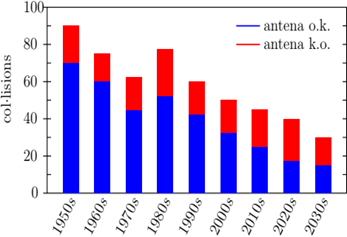
\includegraphics[width=0.5\linewidth]{img/example.png}
    \caption[Shorter name for list of tables or to escape the citation]{Caption below the image \cite{dawson}.}
    \label{fig:graph}
\end{figure}

Phasellus venenatis leo vitae sagittis aliquam. Fusce fringilla fringilla pharetra. Maecenas ac libero nec augue feugiat consectetur. Suspendisse potenti. Integer eget enim tincidunt risus aliquam dignissim in nec sem. Suspendisse ultrices hendrerit fringilla. Duis in nibh venenatis, blandit diam id, feugiat nisi. Mauris fermentum maximus dui nec accumsan. 

\begin{table}[htbp!]
    \centering
    \renewcommand{\arraystretch}{1.07}
    \begin{tabular}{@{}lccr@{}}
        \toprule
        \bfseries Dècada & \bfseries Antena ok & \bfseries Antena ko & \bfseries Total\\
        \midrule
        1950s & 70 & 20 & 90\\
        1960s & 60 & 18 & 78\\
        1970s & 44 & 21 & 63\\
        \bottomrule
    \end{tabular}
    \caption[Shorter name]{Caption below the table.}
    \label{tab:example}
\end{table}

\section{Bibliography}

The UPC recommends using the IEEE style, which this template uses. This is achieved with the \verb+biblatex+ and \verb+biblatex-ieee+ packages. Add your sources to \verb+references.bib+ following the biblatex scheme with whatever fields, and the style will determine which ones to show.

Most journal publishers feature a button to export the citation to BibTeX, usually under ``Cite" (e.g., ScienceDirect) or ``Tools" (e.g., Wiley). In that case, you can just copy the content of the .bib file to \verb+references.bib+. If there is no button or you aren't referencing a journal article, use the usual biblatex syntax.

In order to follow the \href{https://journals.ieeeauthorcenter.ieee.org/wp-content/uploads/sites/7/IEEE_Reference_Guide.pdf}{IEEE style} more closely, do the following:

\begin{outline}
    \1 If the reference has a DOI number, use the \verb+doi+ field in favor of the \verb+url+ field (i.e., delete the latter).
    \1 If the reference is recorded in a database that uses HDL, you can cite it like so:
    \2[] \verb+eprinttype = {hdl}, eprint={XXXXX/XXX}+
    \1 If a journal uses article numbers instead of pages, use the field \verb+eid+ instead:
    \2[] \verb+eid = {XXX}+
    \1 References to Bachelor's and Master's theses can be generated with the \verb+@mastersthesis+ entry type; remember to set the \verb+type+ to \verb+B.S. thesis+ or \verb+M.S. thesis+ accordingly.
    PhD dissertations are usually cited as \verb+@phdthesis+. 
    \1 The IEEE style calls for article or book titles to be in sentence case, that is, only the first letter of the title and proper names. However, the \LaTeX\ implementation converts them to lowercase indiscriminately; you can prevent this by surrounding the affected word with curly brackets \verb+{}+.
\end{outline}

Examples:
\begin{outline}
    \1[] Yada yada yada \cite{incollection}; \textcite{articlelargepages} stated that...; this has solid evidence \cite{dawson,ieec,bookwitheditor}. \nocite{Li2007}
\end{outline}

\section{Code listings and algorithms}

The EETAC style guide gives no direction on formatting algorithms, code snippets, or listings, so I took some liberties without straying much from the general style. Therefore, you can tweak these as you like.

{\centering
\begin{minipage}{.7\linewidth}
    \begin{algorithm}[H]
        \begin{algorithmic}[1]
            \Procedure{Euclid}{$a,b$}\Comment{The g.c.d. of a and b}
            \State $r\gets a\bmod b$
            \While{$r\not=0$}\Comment{We have the answer if r is 0}
            \State $a\gets b$
            \State $b\gets r$
            \State $r\gets a\bmod b$
            \EndWhile\label{euclidendwhile}
            \State \textbf{return} $b$\Comment{The gcd is b}
            \EndProcedure
        \end{algorithmic}
        \caption{Euclid's algorithm}
        \label{euclid}
    \end{algorithm}
\end{minipage}
\par
}

\begin{listing}[htbp!]
    \label{code:example}
    \inputminted[]{python}{img/example.py}
    \captionof{listing}{Some example code} 
\end{listing}


% Bibliography
\printbibliography[title=References,heading=bibliography]
\addcontentsline{toc}{chapter}{References}

\begin{appendices}
    \renewcommand\appendixname{Annex}
    
    \chapter{Example}

Lorem ipsum dolor sit amet, consectetur adipiscing elit. Etiam efficitur a sem a mattis. Quisque tellus nunc, accumsan eget dignissim quis, condimentum eu mi. In sem magna, lacinia non commodo id, laoreet id dolor. Nunc dictum ut tellus eget laoreet. Donec et sem massa. Mauris eu volutpat mauris, ut blandit leo. Orci varius natoque penatibus et magnis dis parturient montes, nascetur ridiculus mus.

\begin{equation}
    \diffp{\vect{B}}{t} = \nabla\times(\vect{v}\times\vect{B})+\frac{\eta}{\mu_0}\nabla^2\vect{B}
\end{equation}

Vestibulum pellentesque pretium nisi, ac venenatis libero aliquet vitae. Sed ornare mi feugiat pharetra accumsan. Ut tincidunt orci at placerat ultricies. Morbi efficitur, ligula sed maximus sollicitudin, nunc ex efficitur urna, efficitur porta ex nisl nec justo. Aenean eu placerat metus. Donec cursus leo ac urna tristique, et convallis dolor hendrerit. In sed leo urna. Suspendisse dignissim elit nec pellentesque volutpat. Nunc nec orci ullamcorper, elementum augue vel, tincidunt odio. Vivamus consequat consequat massa. Nulla vulputate augue in neque feugiat dignissim. Sed maximus vestibulum lectus nec gravida. Praesent non molestie libero. Donec commodo ante vel justo tempus, eget tincidunt justo congue. Nulla tellus est, vehicula eget tincidunt at, dignissim sit amet purus.

    \cleardoublepage
    \begin{landscape}
\chapter{Sustainability and ethical implications analysis}

The current UPC thesis guidelines enforce that all Bachelor's and Master's theses shall include a section where the environmental and social impact of the thesis is estimated. More information can be found \href{https://govern.upc.edu/ca/consell-de-govern/consell-de-govern/sessio-07-2023-del-consell-de-govern/comissio-docencia-i-politica-academica-pendent-celebracio/informacio-de-la-guia-per-incorporar-lanalisi-de-sostenibilitat-i-implicacions-etiques-en-els-tfe/informacio-de-la-guia-per-incorporar-lanalisi-de-sostenibilitat-i-implicacions-etiques-en-els-tfe/@@display-file/visiblefile/Guia%20Informe%20Sostenibilitat%20TFG_TFM_versi%C3%B3%20UPC.pdf}{here} (in Catalan). You can follow the ``matrix" layout or write it out.

\hspace*{\fill}\vspace*{\fill}

%\begin{landscape}
    \begin{table}[htbp!]
        \centering
        \footnotesize
        \renewcommand{\arraystretch}{1.07}
        \begin{tabular}{@{}lm{6.5cm}m{7cm}m{5.5cm}@{}}
            \toprule
             & \bfseries Project development & \bfseries Exploitation & \bfseries Risks and limitations\\
            \midrule
            \bfseries Environmental & Quantify the environmental impact of the project. What measures have you taken to reduce the impact? Have you quantified this reduction? Does your design follow the cradle-to-cradle philosophy? · What is the origin of the raw materials and/or materials used? Do your suppliers publish environmental reports? · Do your suppliers follow the RoHS directive? Do your suppliers follow the RBA Code of Conduct? & What resources do you estimate will be used during the project's lifetime? What will be the environmental impact of these resources? · Will the project reduce the use of other resources? Overall, will the use of the project improve or worsen the ecological footprint? · When the life of the project comes to an end, what waste is generated? How the environmental impact of dismantling can be reduced? · Could the project be carried out with less environmental impact? & Could any scenarios that might increase the footprint of the project arise? · If you did the project again, could it be done with fewer resources? Can it be designed again with reused materials? · What have been the main limitations of the environmental analysis of your proposal?\\
            \midrule
            \bfseries Economic & Quantify the project's cost (human and material resources). What decisions have you taken to reduce the cost? Have you quantified the savings? · Is the estimated cost similar to the final cost? Justify the differences (lessons learned). & What is the estimated cost of the project over its lifetime? Could this cost be reduced to make the project more feasible? · Have you considered the cost of adjustments, updates, or repairs over the life of the project? · Would the dismantling of the project incur any additional costs? · Could any other project benefit from the results of this one? & Could any scenarios arise that may jeopardize the viability of the project? · What have been the main limitations of the economic analysis of your proposal?\\
            \midrule
            \bfseries Social & Does this project involve significant reflections on the personal, professional, or ethical standards of the people working on the project? Has inclusive and non-sexist language been used? · What is the sector's current situation related to the project? · Do the distributors, manufacturers, suppliers, and retailers meet public ethical or conduct codes? & Who benefits from the use of the project? Is there any group that may be adversely affected by the project? If so, to what extent? · To what extent does the project solve the problem initially raised? · Are there other ways of implementing the project that lead to different social impacts? · Does the project avoid biases, stereotypes, and gender roles? · Have you considered the usability of your product for people with diverse needs (age, gender, sex, functional diversity, cultural diversity, etc.)? Are there barriers to using it? & Could any scenarios arise to make the project detrimental to any particular segment of the population? · Could the project create any dependency that might leave users in a weak position? · What have been the main limitations of the social analysis of your proposal?\\
            \bottomrule
        \end{tabular}
        \caption{Sustainability matrix.}
        \label{tab:seia}
    \end{table}
\end{landscape}
\end{appendices}

\end{document}